conexións\chapter{Fundamentos tecnolóxicos}
\label{chap:fundamentos_tecnoloxicos}

\lettrine{N}{este} capítulo esbozaremos unha arquitectura do sistema e estudaremos as opcións de tecnoloxías dispoñibles para implementalo.

\section{BiekeGuard}

BikeGuard será o nome que asignaremos o sistema e se comporá de dous elementos principais BikView, o dispositivo de control e visualización e BikeCam o dispositivo de captura de imaxes e sinalización lumínica, plantexarase unha variación de este, BikeLed, que so contará con elementos de iluminación, figura~\ref{fig:bikeguard}.

\begin{figure}[tb]
  \centering
  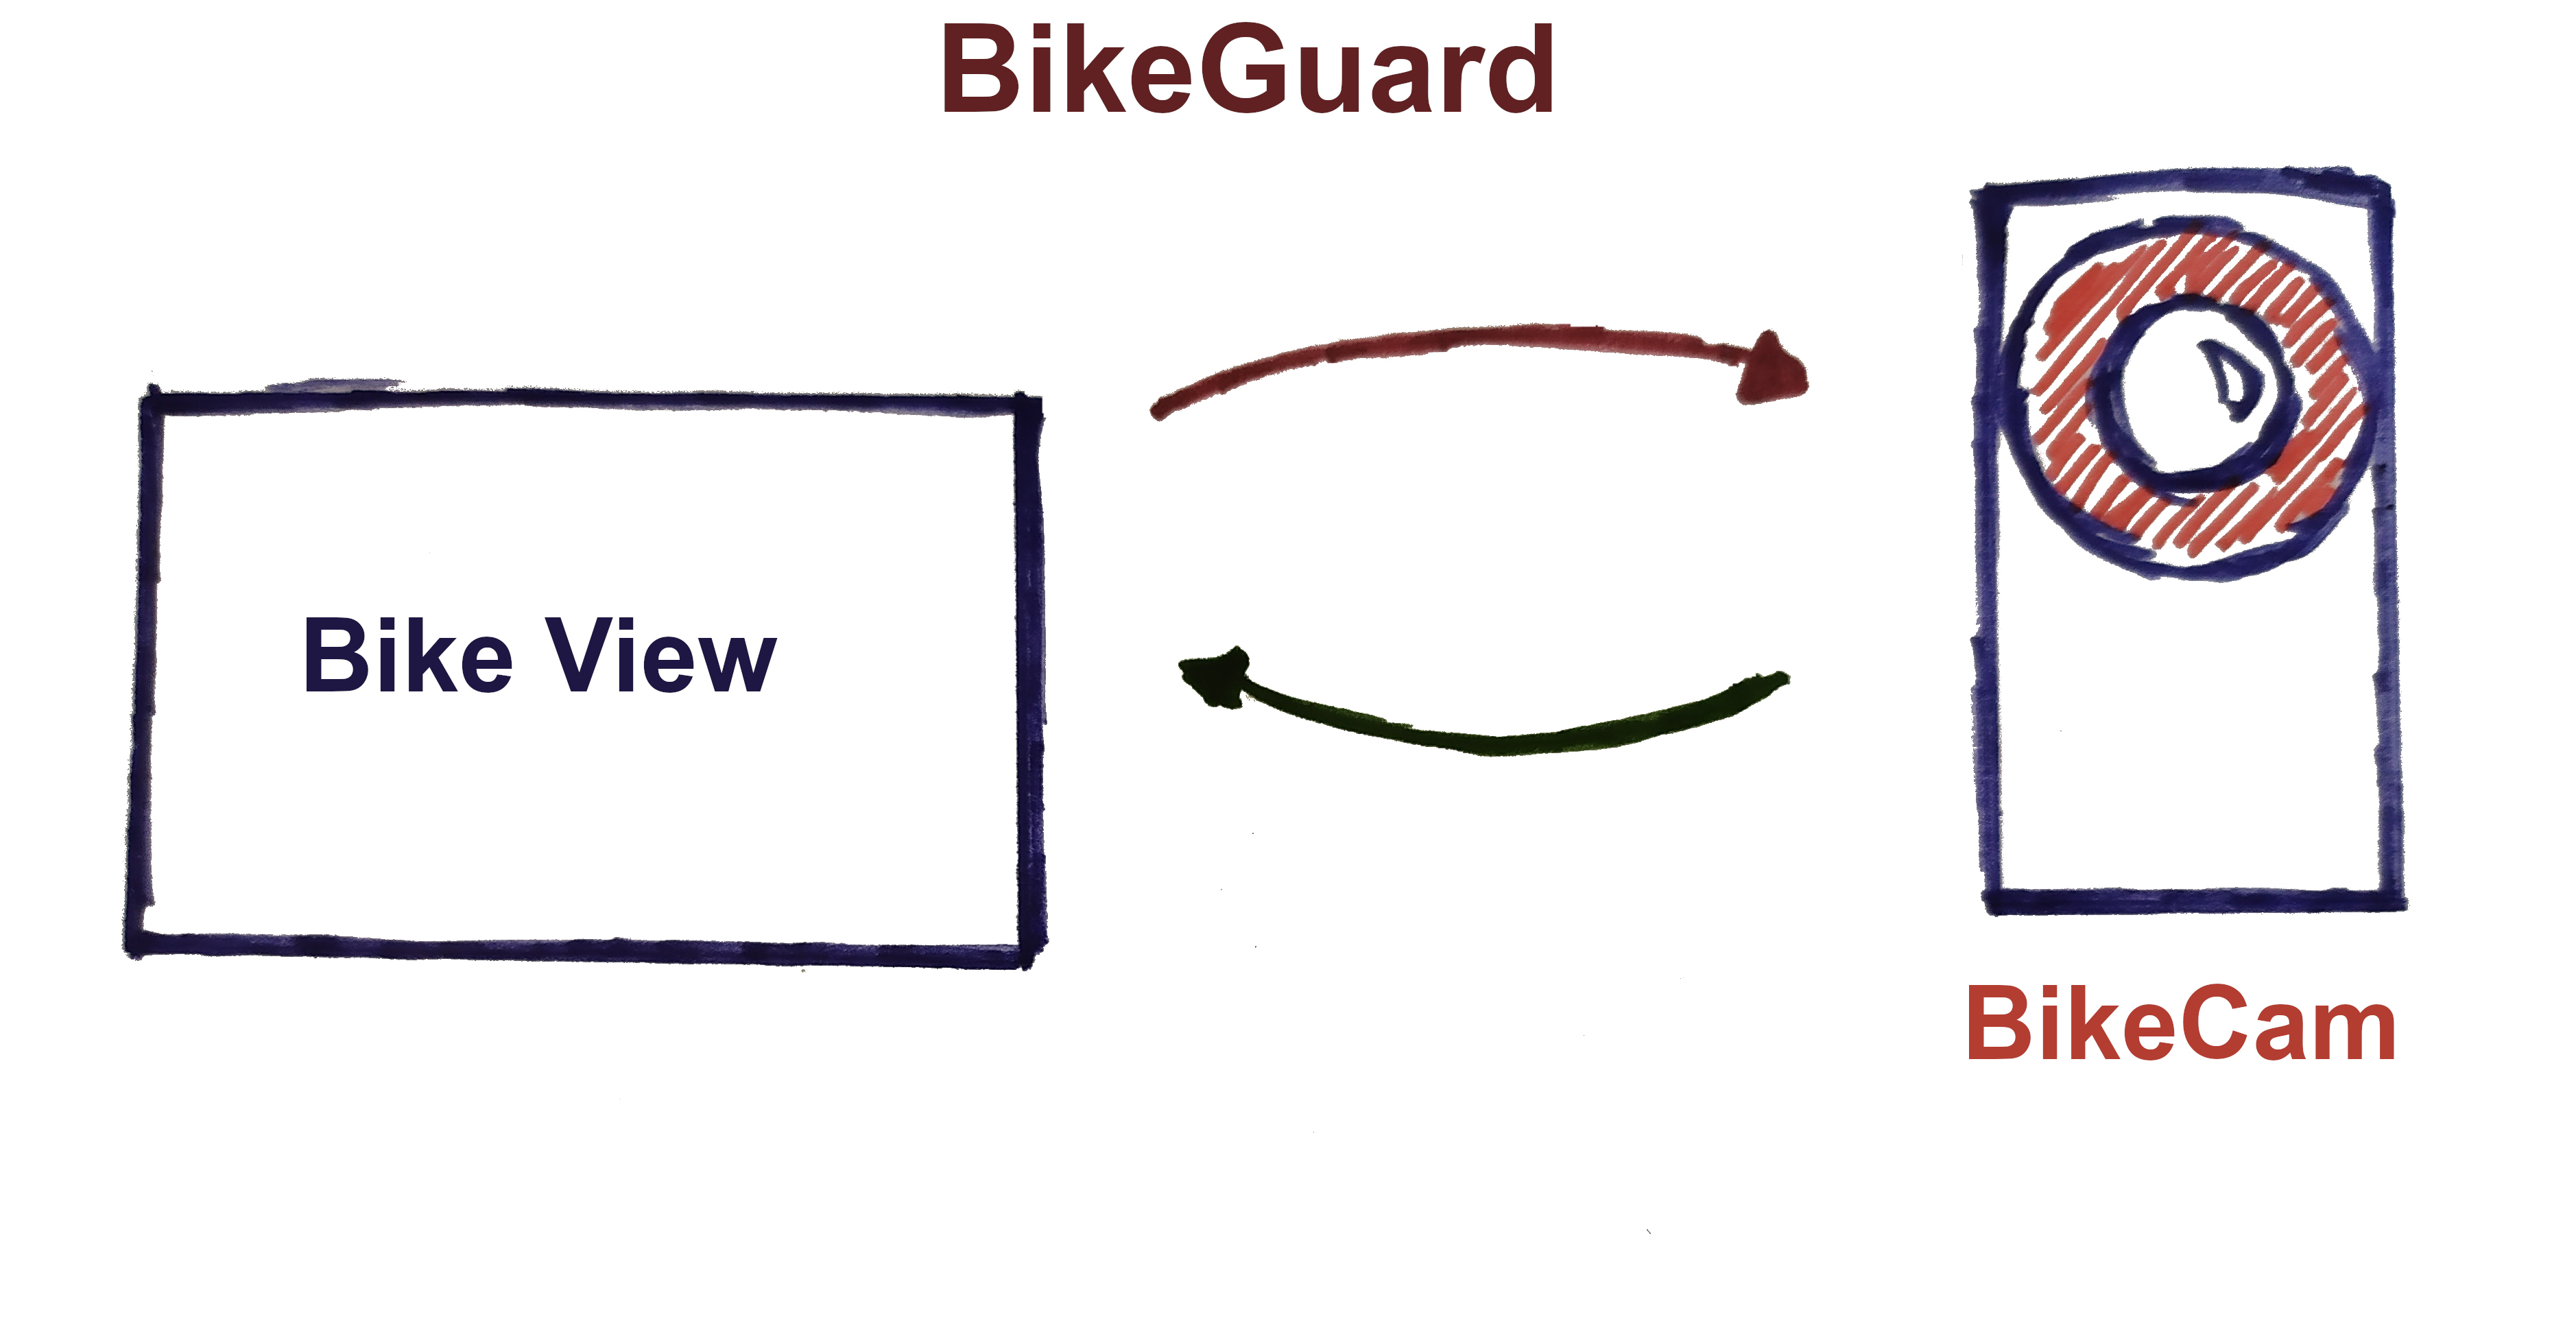
\includegraphics[scale=0.1]{imaxes/bikeguard.jpg}
  \caption{Esquema do sistema BikeGuard.}
  \label{fig:bikeguard}
\end{figure}

Nas seguintes seccións analizaremos as alternativas para o desenvolvemento dos dous dispositivos as conexións entre ambos.

\section{Esquema xeral de BikeView}

Son moitas as posibilidades de implementación deste dispositivo, os requisitos principais son:
\begin{itemize}
    \item Dispoñer dunha pantalla para visualizar o vídeo e o estado das luces.
    \item Contar con algunha interface de entrada de datos como botóns ou pantalla táctil.
    \item Dispoñer dun hardware para comunicarse co dispositivo principal. Como por exemplo: Wi-Fi, Bluetooth ou USB.
    \item Contar cunha batería ou fonte de alimentación
\end{itemize}

Realizar unha implementación física do dispositivo contaría coas vantaxes de poder contar cunha alta personalización dos seus compoñentes e robustez ao contar cun único hardware obxectivo, unha destas opción sería utilizar un miniordenador como a Rasperry Pi conectado a unha pantalla táctil. Sen embargo optarase outra opción moito máis atractiva: utilizar un telefono móbil e crear unha aplicación dende onde poder visualizar o vídeo e controlar as luces aparte de aforrar a construción do dispositivo. Reducirase así o número de compoñentes que o usuario ten que levar, xa que é habitual dispoñer dun móbil en todo momento.

Desenvolverase a aplicación para o sistema operativo Android xa que este é o sistema operativo máis empregado globalmente e nos permitirá chegar a un maior numero de usuarios.

Para suxeitar un teléfono móbil ao guiador da bicicleta existen múltiples ancoraxes que se adaptan a varios tamaños de teléfono. Tamén existen modelos configurables segundo o tamaño do teléfono que despois se poden imprimir en 3D.



\section{Esquema xeral de BikeCam}


As esixencias principais destes dispositivo son a existencia de conexións para as luces leds, conexións para unha cámara e capacidade de procesamento e comunicación o que engadiremos unha quinta esixencia, xa que o obxectivo do proxecto e conseguir unha solución de hardware e software libre que posibilite que o usuario final poida adquirir os compoñentes e montalos de forma sinxela, é preciso que os compoñentes sexan fáciles de adquirir e traballar con eles.

A continuación analizaranse as diferentes opción de hardware dispoñibles, as súas características e seus pros e contras para o proxecto proposto.

\subsection{Placas de desenvolvemento}


Sendo o desenvolvemento dunha placa dedicada a este propósito a solución idílica, o custo de este proceso xunto coa dificultade final da construción, sempre que non se optase por unha produción en serie, son as principais contras desta opción. Poren optarase por elixir unha placa cos requisitos requiridos entre as posibles opcións dispoñibles no mercado. Centrarémonos nos modelos co menor tamaño posible.

As placas contempladas son as seguintes:

\begin{itemize}
    \item Arduino

Arduino é unha compañía dedicada o deseño e produción de placas de desenvolvemento con software e hardware, o que permite que terceiras compañías produzan as súas placas permitindo prezos finais de produto moi baixos.

Con un ide propio cunha linguaxe de programación baseada en C++, cunha ampla compatibilidade con diverso hardware, a diversidade de opcións e a sua facilidade de uso converte as súas placas nas máis populares do mercado.

Polo seu tamaño e forma as placas Arduino consideradas son as seguintes:
    \begin{itemize}
        \item Arduino Micro e Arduino Nano

O primeiro esta baseado no microcontrolador de 8bits ATmega32U4 cunha frecuencia de 16MHz, 32KB de memoria flash e 2.5KB de \emph{SRAM}.
Conta con 20 pins de entradas/saídas dixitais con 7 canles \emph{PWM} e 12 pins de entradas analóxicas.

O segundo baséase no microcontrolador de 8bits ATmega328 traballando a unha frecuencia de 16MHz, conta con 32KB de memoria flash e 2KB de \emph{SRAM}. Conta con 22 pins de entradas/saídas dixitais dos cales 6 son \emph{PWM} tamén conta con 8 pins de entradas analóxicas.

Estas dúas versión o contar con gran cantidade de pins tanto dixitais como analóxicos e un consumo enerxético e moi baixo xunto cun baixo prezo inferior os 5 euros nas versións de fabricantes de terceiros fainos perfectos para o propósito de control de leds, pero a sua baixa potencia computacional dificultaría o procesamento de vídeo. Tampouco conta co hardware necesario para as comunicación sen fíos.

        \item Arduino MKR ZERO e Arduino MKR1000

Ambos baseado no procesador ARM M0+ de 32 bit de baixo consumo cunha frecuencia de funcionamento de 48MHz, 256KB de memoria flash e 32kB de \emph{SRAM}, contan con 7 entradas analóxicas e 1 saída analóxica e 12 pins poden funcionar como PWM. Inclúe conexións \emph{SPI} \emph{UART} e \emph{I2C}. Tamén inclúen unha conexión para alimentalos directamente cunha batería de 3.7v. A diferencia entre ambos e que o primeiro conta con 22 pins de entrada e saída dixital mentres que o segundo conta con 8 pero inclúe un chip Wi-Fi.

Ambos teñen as capacidades de procesamento necesarias para a xestión das luces, do vídeo e as conexións. O único punto negativo é que as cámaras compatibles a nivel de conexión e librerías con estas placas non dispoñen de moita calidade de vídeo.

Estas placas poden obterse por entre 20 e 50 euros

        \item Arduino MKR VIDOR 4000

Esta placa de desenvolvemento a parte do procesador ARM M0+ inclúe un chip \emph{FPGA} que permite a sua configuración como diferentes hardware permitido que a placa poda dispoñer de diferentes compoñentes configurables como podería ser múltiples USB ou chips aceleradores de vídeo. Aparte conta con conexión micro HDMI mini PCI Express e un conector de cámara \emph{MIPI} no que se poderían conectar diversas cámara con calidade máis que suficiente para este proxecto.

O seu prezo e superior os 60 euros.
    \end{itemize}
    \item Raspberry Pi

As Raspberry Pi son unha serie de placas de desenvolvemento cun prezo moi axustado e unha potencia suficiente para para pode executar un sistema operativo completo. Grazas a sua popularidade dispón dun amplo soporte e compatibilidade con diversos software e outras plataformas hardware que a fan perfecta para diversos proxectos, como robótica, \emph{IoT} ou centros multimedia.
A versión dispoñible con menor tamaño e a Raspberry Pi Zero
    \begin{itemize}
        \item Raspberry Pi Zero e Raspberry PI Zero W

Esta placa conta cun microprocesador baseado na arquitectura ARM de 32bits que funciona a 1GHz, acompañase de un procesador de vídeo e unha memoria ram de 512MB. No apartado de conexións conta con un micro USB de carga e outro de datos, unha saída de vídeo HDMI e outra analóxica, unha rañura para unha tarxeta micro sd e un conector de cámara CSI. Tamen conta con 20 pins de conexión que a dotan de entradas e saídas dixitais, dúas canles \emph{PWM}, conexiós \emph{SPI} \emph{I2C} e \emph{UART} xunto a conexións de 5v, 3.3v e terra. A versión Zero W tamén dispón dun chip Wi-Fi e Bluetooth.
A sua potencia e capacidade de conexión a fan máis que capaz de para este proxecto, e o seu prezo, 5 e 10 euros respectivamente, é unha das súas principais vantaxes.
    \end{itemize}
    \item ESP8266 e ESP32

A principal característica destas placas é que implementan chips Wi-Fi e Wi-Fi máis Bluetooth respectivamente,contan cun procesador \emph{RISC} de un ou dous núcleos con velocidades dispoñibles entre os 80MHz e 240MHz e memorias ram de entre 32KiB e 520KiB.

Os seus múltiples portos e interfaces,\emph{SPI} ,  \emph{I2C}, \emph{UART}, \emph{PWM} entre outros, o seu baixo consumo e a sua compatibilidade co entorno de programación de arduino fainos ideais para pequenos proxectos de \emph{IoT}, robótica ou domótica. Segundo as súas características poden obterse dende o prezo de un euro.

O igual que pasaba coas placas Arduino os ESP son ideais para a parte do manexo das luces pero non para a xestión do vídeo. Estudarase como opción para a implementación do dispositivo BikeLed.
    \item Outras placas baseadas en procesadores ARM

NO mercado existen múltiples placas de desenvolvemento baseadas en procesadores ARM, non obstante o prezo e o soporte da Raspberry Pi faina a mellor opción para a maioría de proxectos máis xenéricos.
    \item Outras placas baseadas en \emph{FPGA}

Os chip \emph{FPGA} permiten un nivel de personalización hardware moi elevado, pero tamén contan cun alto prezo, e na maioría dos casos cun \emph{toolchain} privativo que e necesario pagar para poder desenvolver en eles. O contrapunto a sua versatilidade é un maior custo de desenvolvemento en comparación con solucións de programación de alto nivel.
\end{itemize}
Tendo en conta o tamaño, a potencia, as conexións dispoñibles e o prezo, decidiuse optar pola Raspberry Pi Zero e Zero W como a placa encargada do control das luces e do vídeo. O dispor esta dunhas características estándar poderíase substituír nun futuro por outro tipo de placa garantido así a modularidade do sistema.

\subsection{Luces led}
As dúas principais vantaxes das luces led fronte a outras formas de iluminación son o se baixo consumo e o seu pequeno tamaño. Estas calidades fainas ideais para un dispositivo portátil coma o que pretendemos construír.
Os requirimentos principais son poder controlar a intensidade dos leds e dispoñer de polo menos un color vermello para indicar a posición e a freada, e un color amarelo ou ámbar para os intermitentes.

Coa intención de miniaturizar se optara por utilizar leds \emph{RGB} que permiten xerar diversas combinacións de cores e así poder utilizar os mesmos leds para as diferentes funcións.
Xa que a Raspberry Pi non conta con saídas analóxicas, utilizaranse as canles \emph{PWM} que permite enviar sinais moduladas en pulsos. A modulación \emph{PWM} permite acender e apagar os leds múltiples veces a unha alta frecuencia a unha velocidade, tan rápidas que o ollo humano percibe como diferentes intensidades lumínicas en función da anchura dos pulsos. En leds \emph{RGB} compatibles o \emph{PWM} tamén se pode utilizar para codificar a cor elixida, e en series de leds conectados e direccionables se pode elixir que led a iluminar e a súa cor e intensidade individualmente, permitindo así controlar un alto numero de leds cunha soa saída \emph{PWM}.

Existen diferentes tipos de leds \emph{RGB} direccionables no mercado, elixiremos o tipo de led en función do seu tipo de conexión, a dispoñibilidade de librerías de software compatibles e coa limitación de que deberán operar a 5v que a voltaxe constante que necesita a Raspberry Pi para funcionar.\\

Os tipos de led direccionables analizados son:
\begin{itemize}
    \item WS2812B e WS2813

Estes leds inclúen un circuíto integrado en cada led que o conectalos en serie permite o control dunha secuencia teoricamente infinita de leds. Cada led conta con tres entradas e tres saídas: voltaxe, terra e datos. A información a pasar os leds se formara cun fluxo de datos a almacenar nun \emph{buffer} en memoria, ocupando a información de cada un 3 bytes, e se pasarán o primeiro led que lerá os primeiros 24 bits coa información da intensidade de cada cor, vermella, verde e azul, e pasará o resto de datos o seguinte led.

Cada led tarda 30 microsegundos en recibir os datos e 50 microsegundos e actualizar a sua cor, o atraso de transmisión entre leds e de 0.5 microsegundos. O consumo máximo de cada led e de 60 mA a 5V.

Os WS2813 engaden unha segunda liña de datos para que se un led deixa de funcionar os seguintes poidan seguir recibindo a información.
    \item SK6812

Estes leds comparten a maioría de características dos WS2812B coa diferencia de que aumenta a sua taxa de refresco a 1.2KHz con respecto os 400Hz dos WS2812B. Tamén engaden unha cuarta cor branca en cada led.

O a nivel de software son compatibles con WS2812B pero as súas diferenzas non permiten a sua interconexión física.
    \item APA102 e APA102C

Estes leds contan cunha interface SPI que conta cunha sinal de datos é outra de reloxo. Isto e para solucionar o problema de sincronización que se poden producir cando os led son manexados dende placas con capacidade de multitarefa sen un \emph{kernel} especifico para entrada e saída a tempo real. Tamén aumenta sua taxa de refresco ata os 19.2kHz.
\end{itemize}

Sendo os leds APA102 superiores en características os outros dous, contan coa desvantaxe de que requiren máis cables de conexión. As súas vantaxes a nivel de velocidade e sincronismo son esencias para a xeración de imaxes ou vídeo pero non para simples animacións como as que utilizaremos neste proxecto. Porén optaremos por utilizar os leds WS2812B e WS2813 ou SK6812.

Este tipo de leds están dispoñibles en diferentes combinacións: leds individuais, tiras flexibles, tiras ríxidas, aneis e matrices. Faremos probas con tiras e aneis de diferentes tamaños.


\subsection{Cámara}

No caso da cámara plantexanse dúas opcións utilizar unha cámara usb ou unha das cámara deseñadas para funcionar coa Raspberry Pi que utilizan a sua conexión \emph{CSI}. Optaremos pola segunda opción xa que unha cámara usb implica un tamaño demasiado grande para o proxecto e ademais non soen estar indicadas para a iluminación de exteriores.

No mercado existen diversos módulos de cámara para a Raspberry Pi pero a maioría están baseados nos Raspberry Pi Camera Module V1 e Raspberry Pi Camera Module V2 a principal diferencia entre ambos e que o primeiro conto con 5 megapixeles mentres o segundo conta con 8 megapixeles e unha notable mellora na calidade de imaxe.\\

As principais diferenzas nos módulos dispoñibles no mercado son:
\begin{itemize}
    \item Tamaño

Existen versións especificas para a Raspberry Pi Zero máis pequenas pero solo do Camera Module V1, as versións normais xa contan cun tamaño moi axustado.

    \item Presenza de filtro infravermello

As cámara soen contar cun filtro de luz infravermella para evitar o \emph{aliassing} que se produce nas cámara xa que as pantallas que utilizamos non están destinadas para emitir infravermellos e os nosos ollos non son capaces de percibilos. As cámaras que non contan con este filtro dan como resultado imaxes máis luminosas e cunha tonalidade violácea. Estas cámara son útiles para entornas exteriores no solpor ou para visión nocturna se se conta con fontes de luz infravermellas.

    \item Tipo de lente

A uso dunha cámara cunha lente curva permite ampliar o campo de visión da cámara, se a lente e demasiado curva se producirá unha distorsión da imaxe nos bordes.

Xa que estas cámaras son todas compatíbeis a nivel de software probaremos diversos tipos con varios tipos de lente xa sexan incorporados ou engadindo unha lente externa.
\end{itemize}




\subsection{Alimentación e baterías}

A Raspberry Pi Zero necesita unha fonte de alimentación que provea de 5V constantes. O seu consumo enerxético varía segundo a carga computacional, o uso do Wi-Fi e o uso da cámara podendo ascender a entorno 300mA.
Os leds tamén funcionarán a 5V cun consumo máximo de 60mA por led, cando emiten luz branca a máxima intensidade.

Plantexamos dúas solución posibles:
\begin{itemize}
    \item Bateria externa USB

Utilizar unha batería usb externa permite dispoñer de altas capacidades que prolongarían o tempo de uso pero implican o uso dun dispositivo a maiores. Outra de desvantaxes e que cando se esgote a batería a corrente interrompese de golpe sen que a Raspberry poida realizar un apagado normal, como consecuencia tras varios apagados podería danarse o sistema de ficheiros se se estaba a escribir nel no momento do apagado.

    \item Batería, circuíto de alimentación e circuíto de acendido e apagado.

A maioría de baterías usadas en electrónica son baterías de \emph{ions de litio} principalmente devido as sua alta capacidade enerxética e lonxevidade. A \emph{voltaxe nominal} destas baterías e de 3.7V sendo 4.2V a voltaxe coa carga o máximo e por debaixo de 3V deixan de proporcionar suficiente intensidade eléctrica para a maioría de aplicacións. Este tipo de baterías son as que atoparemos nos teléfonos móbiles, ordenadores portátiles e incluso en vehículos eléctricos. Poden colocarse en serie cando e necesario unha maior voltaxe ou en paralelo cando o que se necesita e unha maior capacidade.

Para poder utilizar estas baterías é necesario un circuíto de carga, un de protección, e un de conversión de voltaxe. Na maioría dos casos as batería de consumo utilizan o estándar USB, que funciona a 5V, tanto para cargarse como para proporcionar enerxía. Polo que será necesario un chip de carga que acepte unha toma de 5V e que cargue a batería ata 4.2V. As baterías de litio poden ser perigosas danándose e chegando incluso a estoupar se se descargan demasiado ou se se sobrecargan polo que é necesario un circuíto de protección que evite a sobrecarga e a sobrecarga. Para proporcionar unha saída estable de 5V tamén é necesario un conversor de voltaxe.
É habitual atopar o circuítos de carga máis protección xuntos no mesmo chip aínda que tamén se atopan circuítos que integran as tres funcionalidades.
\end{itemize}
\subsection{Software a utilizar}
A Raspberry Pi conta cunha ampla gama de sistemas operativos, algúns con propósitos concretos como reprodución de multimedia, servidores locais ou nodos de rede. Tamén conta con versións das distribucións Linux máis popular como Ubuntu, Arch ou Kali entre outros.
Raspbian é unha distribución baseada en Debian, é máis antiga e máis optimizada para a Raspberry Pi e a que dispón de máis soporte polo que será a elixida para o proxecto.

Para o control dos leds existen varias librarías dispoñibles para varias linguaxes de programación. As máis utilizadas son a de Adafruit, que só está dispoñible en Python, e a de Jeremy Garff que será a que utilicemeos, xa que conta con unha documentación detallada e esta dispoñible en varias linguaxes de programación, entre outras C, Python e Java.

Para a captura e transmisión do vídeo contamos con varias alternativas. A libraría \emph{picamera} para Python permite configurar calquera parámetro e o \emph{streaming} do vídeo na rede. Por outra parte o software para captura de vídeo \emph{raspivideo}, escrito en Python, tamén permite moitos parámetros de configuración é a sua saída de vídeo pode enviarse a rede utilizando algún programa para redirecionar o \emph{bitstream} dos datos como pode ser o software \emph{socat}.

A comunicación entre o dispositivo de control e o de luces e captura de vídeo realizarase a través dunha conexión IP. Para manexar as peticións podemos empregar unha das clases servidor Python, unha libraría de terceiros ou implementar o servidor a nivel de \emph{sockets}.

Por motivos de compatibilidade entre todo o software necesitado para o control de leds, vídeo, e conexións, decidiremos integralo todo nunha aplicación Python que se encargará das tres tarefas.

\subsection{Caixa e ancoraxes a bicicleta}


O lugar a colocar o dispositivo de iluminación e captura será na barra da sela da bicicleta, esta posición é a ideal tanto para capturar o vídeo como para que as luces sexan vistas polo tráfico que circula detrás do vehículo.

A Raspberry Pi conta cunha caixa oficial na que se pode instalar xunto coa cámara V2. Esta é a que utilizaremos no caso de alimentala cunha batería externa. Para suxeitar a placa á barra deseñaremos un soporte e o imprimiremos cunha impresora 3D. Para a versión con batería interna deseñaremos unha caixa protectora que albergue tódolos compoñentes e que se poida suxeitar á barra.

Os prototipos imprimiranse en \emph{PLA} un material biodegradable e de fácil impresión, no é o mellor material para resistir a auga ou a humidade pero é ideal para o prototipado. Poderá utilizarse \emph{ABS} para imprimir unha versión final, un material moito máis resistente as condicións atmosféricas.

\section{Conexión entre BikeView e BikeCam}
Optarase por utilizar un sistema de conexión cliente servidor no que BikeView realizara peticións o servidor en BikeCam que responderá actuando as luces e devolvendo cofirmacións e a sinal de video.

Partindo da elección da Raspebrry Pi para BikeCam e un dispositivo Android para BikeView as opcións para a implementación física da conexión son as seguintes.

\subsection{USB}
A Raspberry Pi Zero conta cun conector USB 2.0, e os dispositivos Android implementan este estándar ou o superior 3.0 polo que a velocidade máxima será restrinxida pola Raspberry Pi permitindo un máximo de 480Mbits/s esta velocidade permitiría a transimisión de vidio sen problemas.
Tanto no dispositivo Android como na Raspberry Pi pódese implementar unha conexión Ethernet virtual sobre USB o que facilitaría a estandarización das comunicacións.

Unha das principais vantaxes de usar unha conexión USB é que poderíase alimentar enerxeticamente o dispositivo BikeCam dende BikeView sempre e cando o consumo de este non supere o máximo de 500mA que pode subministrar un dispositivo Android por USB en modo OTG.

A principal desvantaxe é a necesidade de ter un cable unindo ambos dispositivos dende o guiador a sela da bicicleta.
\subsection{WI-Fi}
A Raspberry Pi Zero conta con un chip WI-Fi 802.11n e calquera móbil actual implementan esta versión do estándar ou unha superior. Este estandar Wi-Fi permite unha velocidade máxima de transmisión de 300Mbits/s tamén neste caso suficiente para a transmisión de vídeo HD.

A principal vantaxe do uso do WI-Fi é a independencia dos dispositivos pero coma contrapartida será necesario que BikeCam conte cunha batería propia.
\subsection{Bluetooth}
Bluetooth 4.0 é a versión do estándar implemetado pola Rasberry Pi Zero W e neste caso tamén marcará a velocidade máxima de transmisión xa que os dispositivos Android actuais implementan versións iguales ou superiores do estándar.Esta velocidade será 25Mbits/s o que non nos permitiría transmitir vídeo en tempo real. Sen embargo esta conexión e máis que suficiente para o dispositivo BikeLed que non require transmisión de vídeo.

Unha das súas vantaxes fronte o Wi-Fi e menor consumo enerxético.

Tendo en conta a viabilidade das tres opción optarase por a implementación das conexión a través de Wi-Fi xa que é a opción que menos limitacións carrexa.
